%%%%%%%%%%%%%%%%%%%%%%%%%%%%% Define Article %%%%%%%%%%%%%%%%%%%%%%%%%%%%%%%%%%
\documentclass{article}
%%%%%%%%%%%%%%%%%%%%%%%%%%%%%%%%%%%%%%%%%%%%%%%%%%%%%%%%%%%%%%%%%%%%%%%%%%%%%%%

%%%%%%%%%%%%%%%%%%%%%%%%%%%%% Using Packages %%%%%%%%%%%%%%%%%%%%%%%%%%%%%%%%%%
\usepackage{fancyhdr}
\usepackage{lastpage}
\usepackage{titling}
\usepackage[danish]{babel}
\usepackage{geometry}
\usepackage{graphicx}
\usepackage{amssymb}
\usepackage{amsmath}
\usepackage{amsthm}
\usepackage{empheq}
\usepackage{mdframed}
\usepackage{booktabs}
\usepackage{lipsum}
\usepackage{graphicx}
\usepackage{color}
\usepackage{xcolor}
\usepackage{psfrag}
\usepackage{pgfplots}
\usepackage{bm}
\usepackage{hyperref}
\usepackage{minted}
\usepackage{svg}
%%%%%%%%%%%%%%%%%%%%%%%%%%%%%%%%%%%%%%%%%%%%%%%%%%%%%%%%%%%%%%%%%%%%%%%%%%%%%%%

% Other Settings

%%%%%%%%%%%%%%%%%%%%%%%%%% Page Setting %%%%%%%%%%%%%%%%%%%%%%%%%%%%%%%%%%%%%%%
\geometry{a4paper, bottom=3cm}


%%%%%%%%%%%%%%%%%%%%%%%%%% Styles %%%%%%%%%%%%%%%%%%%%%%%%%%%%%%%%%%%%%%%%%%%%%
\usemintedstyle{borland}
%%%%%%%%%%%%%%%%%%%%%%%%%% Define some useful colors %%%%%%%%%%%%%%%%%%%%%%%%%%
\definecolor{ocre}{RGB}{243,102,25}
\definecolor{mygray}{RGB}{243,243,244}
\definecolor{deepGreen}{RGB}{26,111,0}
\definecolor{shallowGreen}{RGB}{235,255,255}
\definecolor{deepBlue}{RGB}{61,124,222}
\definecolor{shallowBlue}{RGB}{235,249,255}
%%%%%%%%%%%%%%%%%%%%%%%%%%%%%%%%%%%%%%%%%%%%%%%%%%%%%%%%%%%%%%%%%%%%%%%%%%%%%%%

%%%%%%%%%%%%%%%%%%%%%%%%%%% Define codecomment command %%%%%%%%%%%%%%%%%%%%%%%%
\newcommand{\code}[1]{\small\mintinline[xleftmargin=2em, xrightmargin=2em,
breaklines]{java}{#1}}
\newcommand{\snippet}[3]{\inputminted[firstline=#1,lastline=#2,linenos,
xleftmargin=1.5em, breaklines]{java}{#3}}
%%%%%%%%%%%%%%%%%%%%%%%%%%%%%%%%%%%%%%%%%%%%%%%%%%%%%%%%%%%%%%%%%%%%%%%%%%%%%%%

%%%%%%%%%%%%%%%%%%%%%%%%%% Define an orangebox command %%%%%%%%%%%%%%%%%%%%%%%%
\newcommand\orangebox[1]{\fcolorbox{ocre}{mygray}{\hspace{1em}#1\hspace{1em}}}
%%%%%%%%%%%%%%%%%%%%%%%%%%%%%%%%%%%%%%%%%%%%%%%%%%%%%%%%%%%%%%%%%%%%%%%%%%%%%%%

%%%%%%%%%%%%%%%%%%%%%%%%%%%% English Environments %%%%%%%%%%%%%%%%%%%%%%%%%%%%%
\newtheoremstyle{mytheoremstyle}{3pt}{3pt}{\normalfont}{0cm}{\rmfamily\bfseries}{}{1em}{{\color{black}\thmname{#1}~\thmnumber{#2}}\thmnote{\,--\,#3}}
\newtheoremstyle{myproblemstyle}{3pt}{3pt}{\normalfont}{0cm}{\rmfamily\bfseries}{}{1em}{{\color{black}\thmname{#1}~\thmnumber{#2}}\thmnote{\,--\,#3}}
\theoremstyle{mytheoremstyle}
\newmdtheoremenv[linewidth=1pt,backgroundcolor=shallowGreen,linecolor=deepGreen,leftmargin=0pt,innerleftmargin=20pt,innerrightmargin=20pt,]{theorem}{Theorem}[section]
\theoremstyle{mytheoremstyle}
\newmdtheoremenv[linewidth=1pt,backgroundcolor=shallowBlue,linecolor=deepBlue,leftmargin=0pt,innerleftmargin=20pt,innerrightmargin=20pt,]{definition}{Definition}[section]
\theoremstyle{myproblemstyle}
\newmdtheoremenv[linecolor=black,leftmargin=0pt,innerleftmargin=10pt,innerrightmargin=10pt,]{problem}{Problem}[section]
%%%%%%%%%%%%%%%%%%%%%%%%%%%%%%%%%%%%%%%%%%%%%%%%%%%%%%%%%%%%%%%%%%%%%%%%%%%%%%%

%%%%%%%%%%%%%%%%%%%%%%%%%%%%%%% Plotting Settings %%%%%%%%%%%%%%%%%%%%%%%%%%%%%
\usepgfplotslibrary{colorbrewer}
\pgfplotsset{width=8cm,compat=1.9}
%%%%%%%%%%%%%%%%%%%%%%%%%%%%%%%%%%%%%%%%%%%%%%%%%%%%%%%%%%%%%%%%%%%%%%%%%%%%%%%

%%%%%%%%%%%%%%%%%%%%%%%%%%%%%%% Title & Author %%%%%%%%%%%%%%%%%%%%%%%%%%%%%%%%
\title{\textbf{Objektorienteret Programmering Projekt PacMan}}
\author{Andreas K. L. \quad Aske W. F. \quad Magnus R. K.}
%%%%%%%%%%%%%%%%%%%%%%%%%%%%%%%%%%%%%%%%%%%%%%%%%%%%%%%%%%%%%%%%%%%%%%%%%%%%%%%

\begin{document}
\pagenumbering{gobble}
\begin{titlepage}
    \maketitle
    \begin{figure}[H]
        \begin{center}
            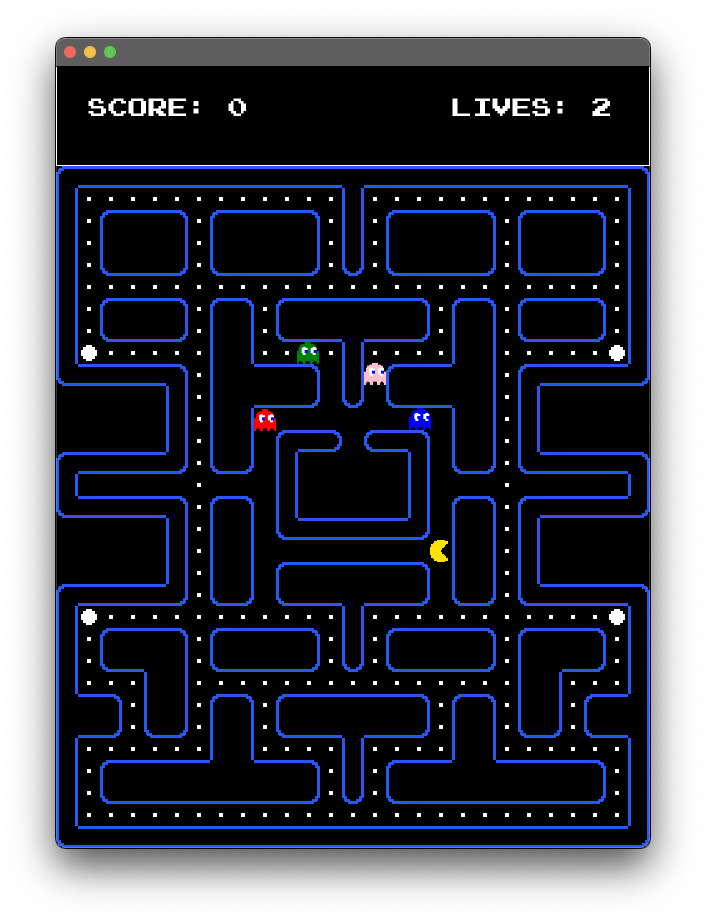
\includegraphics[width=0.77\textwidth]{figures/FrontPageImage.png}
        \end{center}
    \end{figure}
\end{titlepage}
    \clearpage
    \newpage
    \pagenumbering{arabic}
    \setcounter{page}{1}

    % Only footer, no header
    \pagestyle{fancy}
    % \fancyhf{} 
    \fancyfoot[C]{\textbf{\thepage}\ of \pageref{LastPage}}
    % \renewcommand{\headrulewidth}{0pt}  

    \tableofcontents
    \newpage
\section{Projektbeskrivelse}\label{sec:Beskrivelse} % (fold)

Til fordel for at sikre en så tro kopi til orignalen som overhovedet muligt, er dette projekts hovedformål, at udvilke spilfunktionalitet mht. kravsspecifikationen. Målet herefter, er at udvide både spillets funktionalitet samt dets brugervenlighed.

Eventuelle afvigelser fra kravsspecifikationen ses dokumenteret/diskuteret i det følgende.
% \begin{itemize}
%   \item Antag, at læseren af jeres rapport har læst kravsspecifikationen fra
%   projektbeskrivelsen i slutningen af dette dokument, og undlad at gentage
%   unødvendige detaljer derfra.
%   \item Formålet med denne sektion er at dokumentere eventuelle afvigelser fra
%   kravsspecifikationen.
%   \item Har I, for eksempel, gjort jer forsimplende antagelser ift.
%   specifikationen? Eller tolket eventuelle tvetydigheder i specifikationen?
%   Tilføjet nye krav? Beskriv hvilke og hvordan I evt. har tolket
%   specifikationen.
%   \item Hold det kort, især hvis I har få afvigelser.
% \end{itemize}
\newpage
% section Beskrivelse (end)

\section{design}\label{sec:design} % (fold)

\begin{figure}[H]
    \begin{center}
        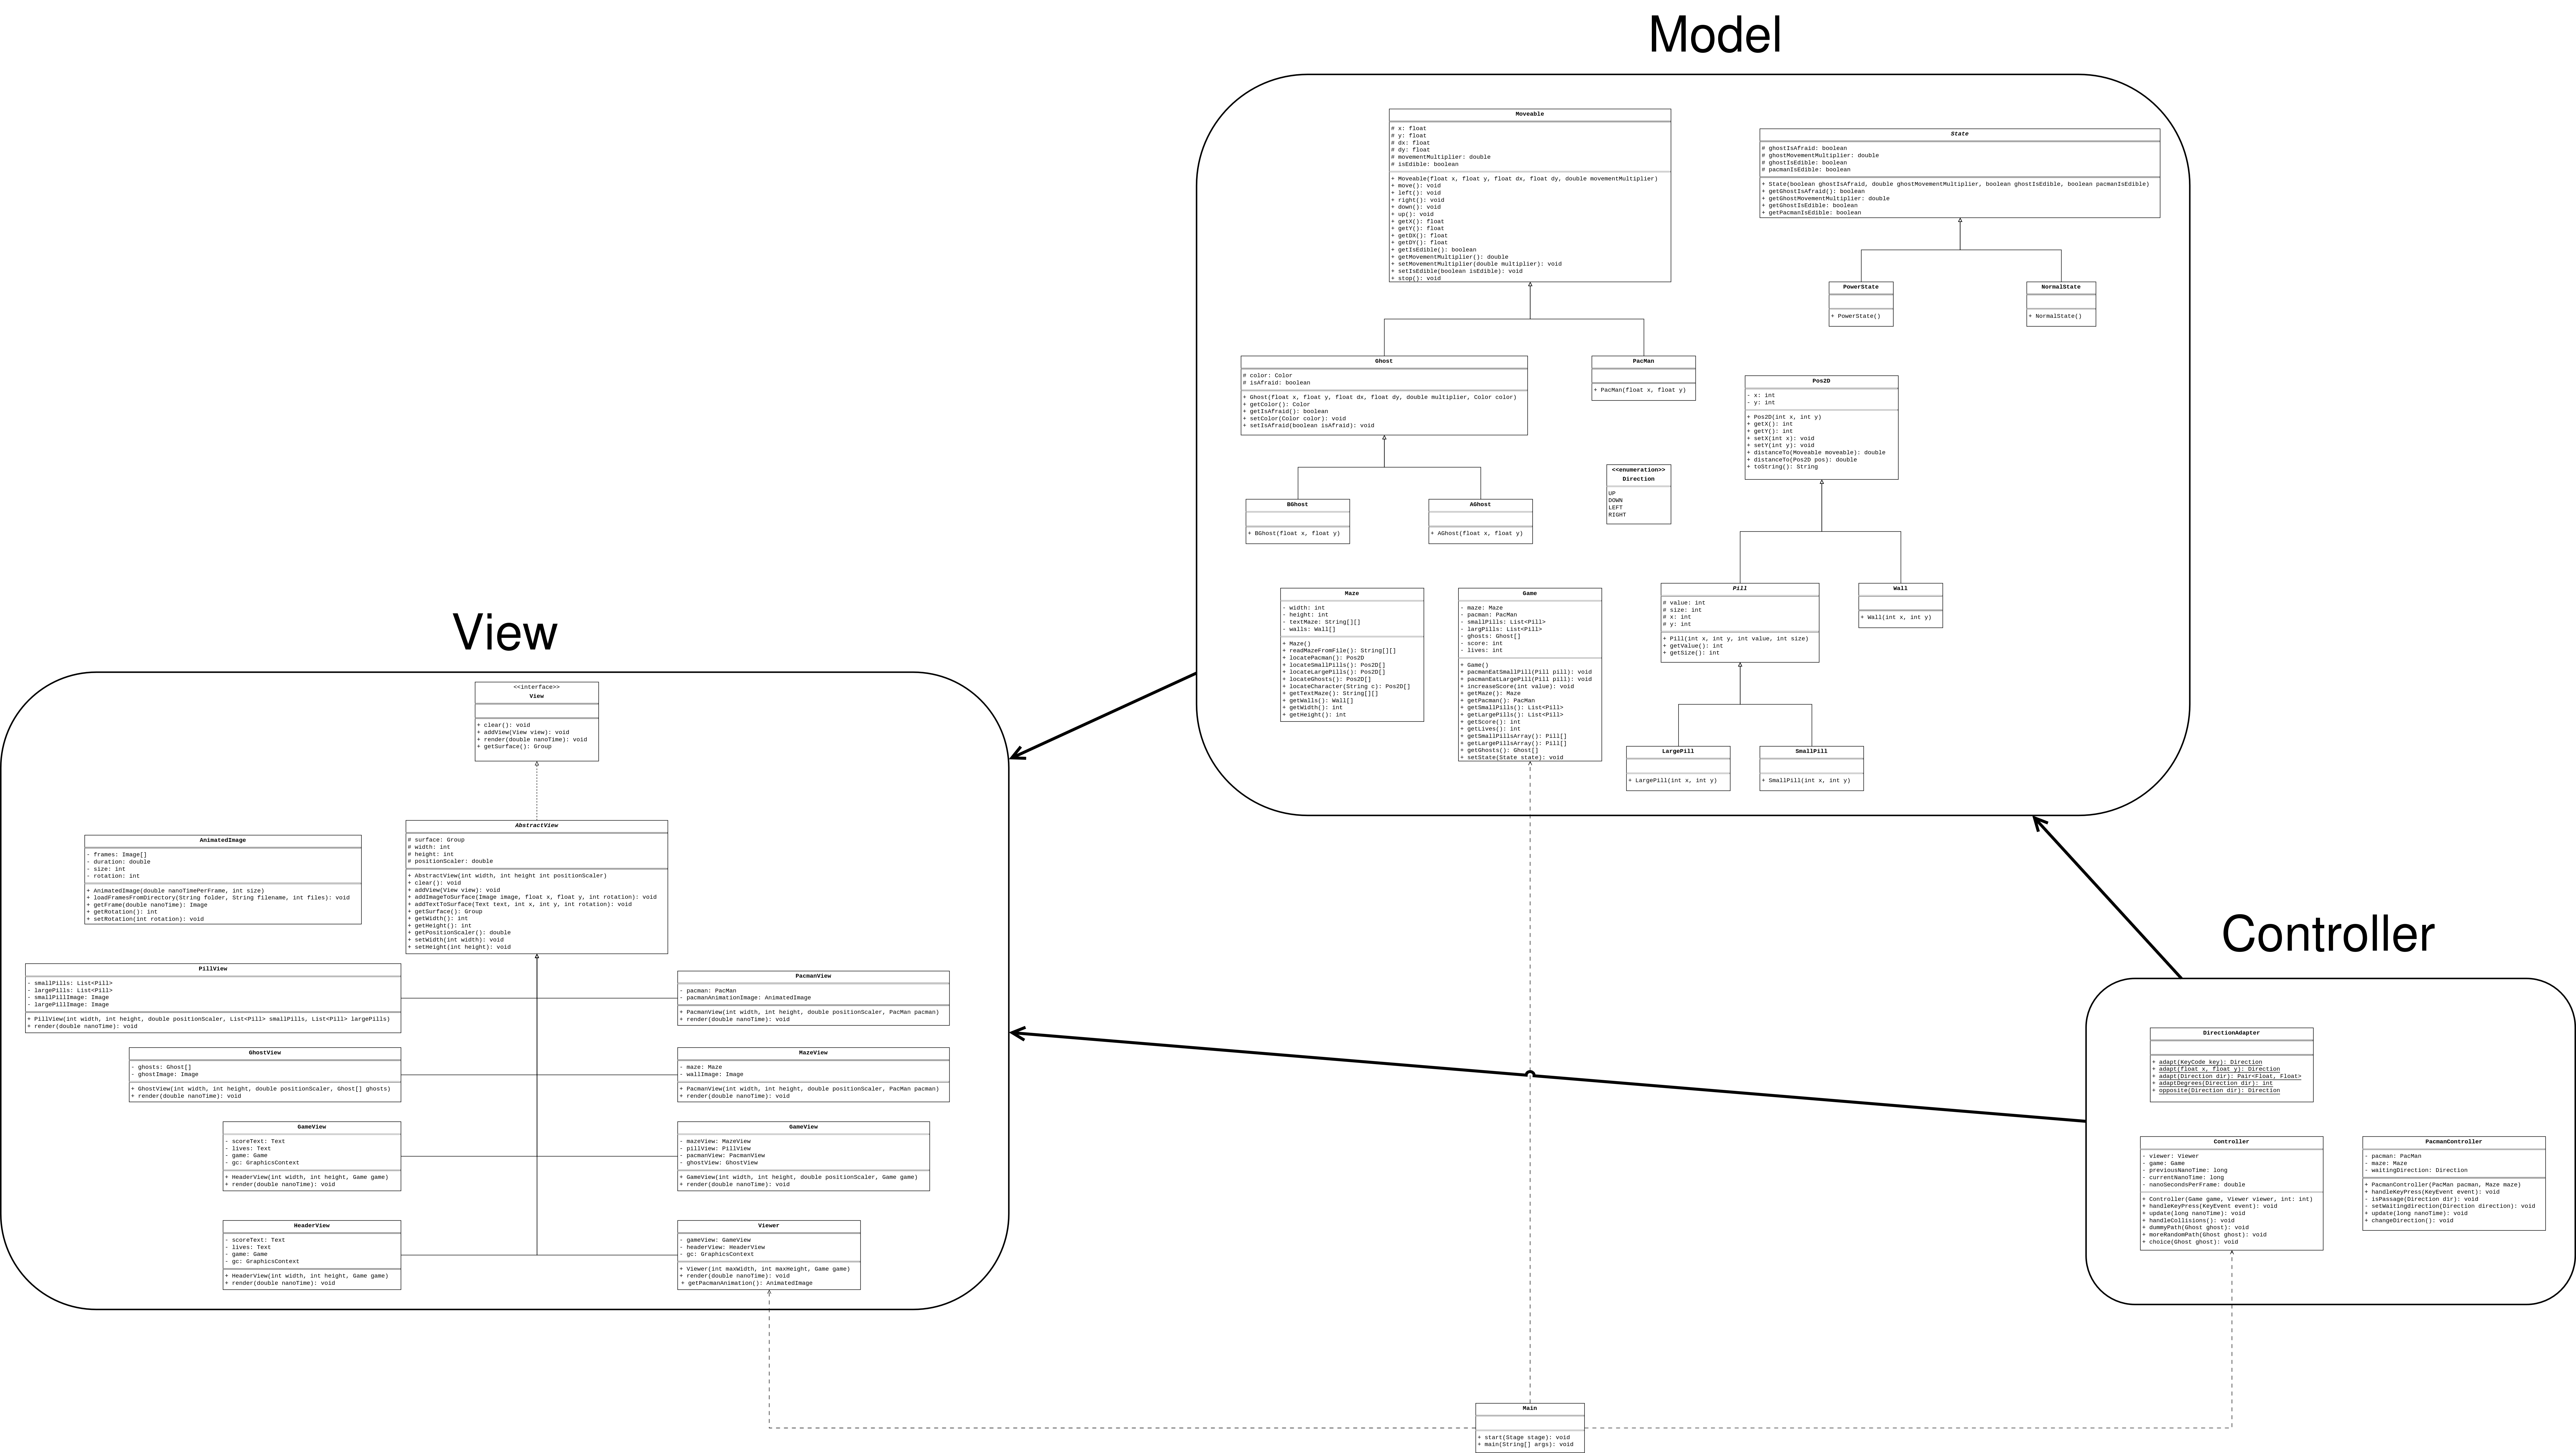
\includegraphics[width=0.95\textwidth]{figures/UML-diagram.png}
    \end{center}
    \caption{}
    \label{UML-diagram}
\end{figure}

Projektets design følger \textit{MVC} (Model-View-Controller) modellen. Det
vil sige at vores \textit{Model} repræsenterer hvordan PacMan spillet er bygget
op med spøgelser, væge, piller osv. Så har vi vores \textit{Controller} som står
for alt logikken med hvordan ting skal kolliderer og bevæge sig, og hvornår de
forskellige stadier af spillet sker. Til sidst har vi vores \textit{View} som
står for at vise spillet, med alle billederne og animationerne, samt score tekst
og liv osv.

Designet kan ses i vores \textit{UML}-diagram, hvor man kan se vi har opdelt
koden i de tre dele fra \textit{MVC} modellen, samt en \textit{main} fil til at
starte spillet, og initialiserer de andre klasser.

Vi har designet alt vores kode med fokus på \textit{indkapslingsprincippet}.
Alle felter i klasser er private, og har kun \textit{getters} og
\textit{setters} der hvor det er nødvendigt. Vi har også overholdt \textit{DRY}
princippet, ved at samle ens opførsel i fælles \textit{superklasser}.


\subsection{Model}\label{sub:Model} % (fold)
\begin{figure}[H]
    \begin{center}
        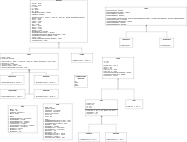
\includegraphics[width=0.95\textwidth]{figures/UML-diagram-model.png}
    \end{center}
    \caption{UML-diagram til \textit{Model} delen af projektet.}
    \label{UML-diagram-Model}
\end{figure}

I \textit{Model} (se \autoref{UML-diagram-Model}) har vi lavet et abstrakt klasse der
hedder \code{Moveable}, som er en abstrakt enhed der kan bevæge sig. Dette
tillader os at \textit{nedarve} fra den når vi skal lave ting der skal bevæge
sig som \code{Ghost} og \code{PacMan}. Ud over dette er \code{Ghost} også en
abstrakt klasse, så vi kan udvide de enkelte spøgelser fra den. Udover
\code{Moveable} klasse, har vi også en klasse, \code{Pos2D}, til at
beskrive positioner som ikke skal kunne bevæge sige. Fra denne klasse kan vi så
nedarve klasser som \code{Pill} og \code{Wall}, da de bare er positioner, men vi
godt vil kunne skelne imellem dem. På denne måde benytter vi
\textit{klasseafhængighedsprincippet} til at simplificerer koden, og gøre det
nemmere at udvide med nye features.
% subsection Model (end)


\subsection{View}\label{sub:View} % (fold)
\begin{figure}[H]
    \begin{center}
        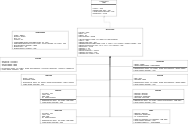
\includegraphics[width=0.95\textwidth]{figures/UML-diagram-view.png}
    \end{center}
    \caption{UML-diagram til \textit{View} delen af projektet.}
    \label{UML-diagram-view}
\end{figure}
I \textit{View} (se \autoref{UML-diagram-view}) har vi benyttet en
\textit{grænseflade} ved navn \code{View} som specificere hvilke metoder et
\textit{View} skal have. Så har vi lavet en abstrakt klasse \code{AbstractView},
som implementerer dette interface. Vi nedarver på denne måde fra det abstrakte
\textit{View} hver gang vi laver et nyt \textit{View} som står for at vise noget
andet. Så kan vi lave specifikke views som står for at tegne kun én slags ting,
f.eks. \code{PacManView}. På denne måde benytter vi princippet om et enkelt
ansvar, svarende til \textit{Single Responsibility Principle} eller \textit{SRP}.
% subsection View (end)

\subsection{Controller}\label{sub:Controller} % (fold)
\begin{figure}[H]
    \begin{center}
        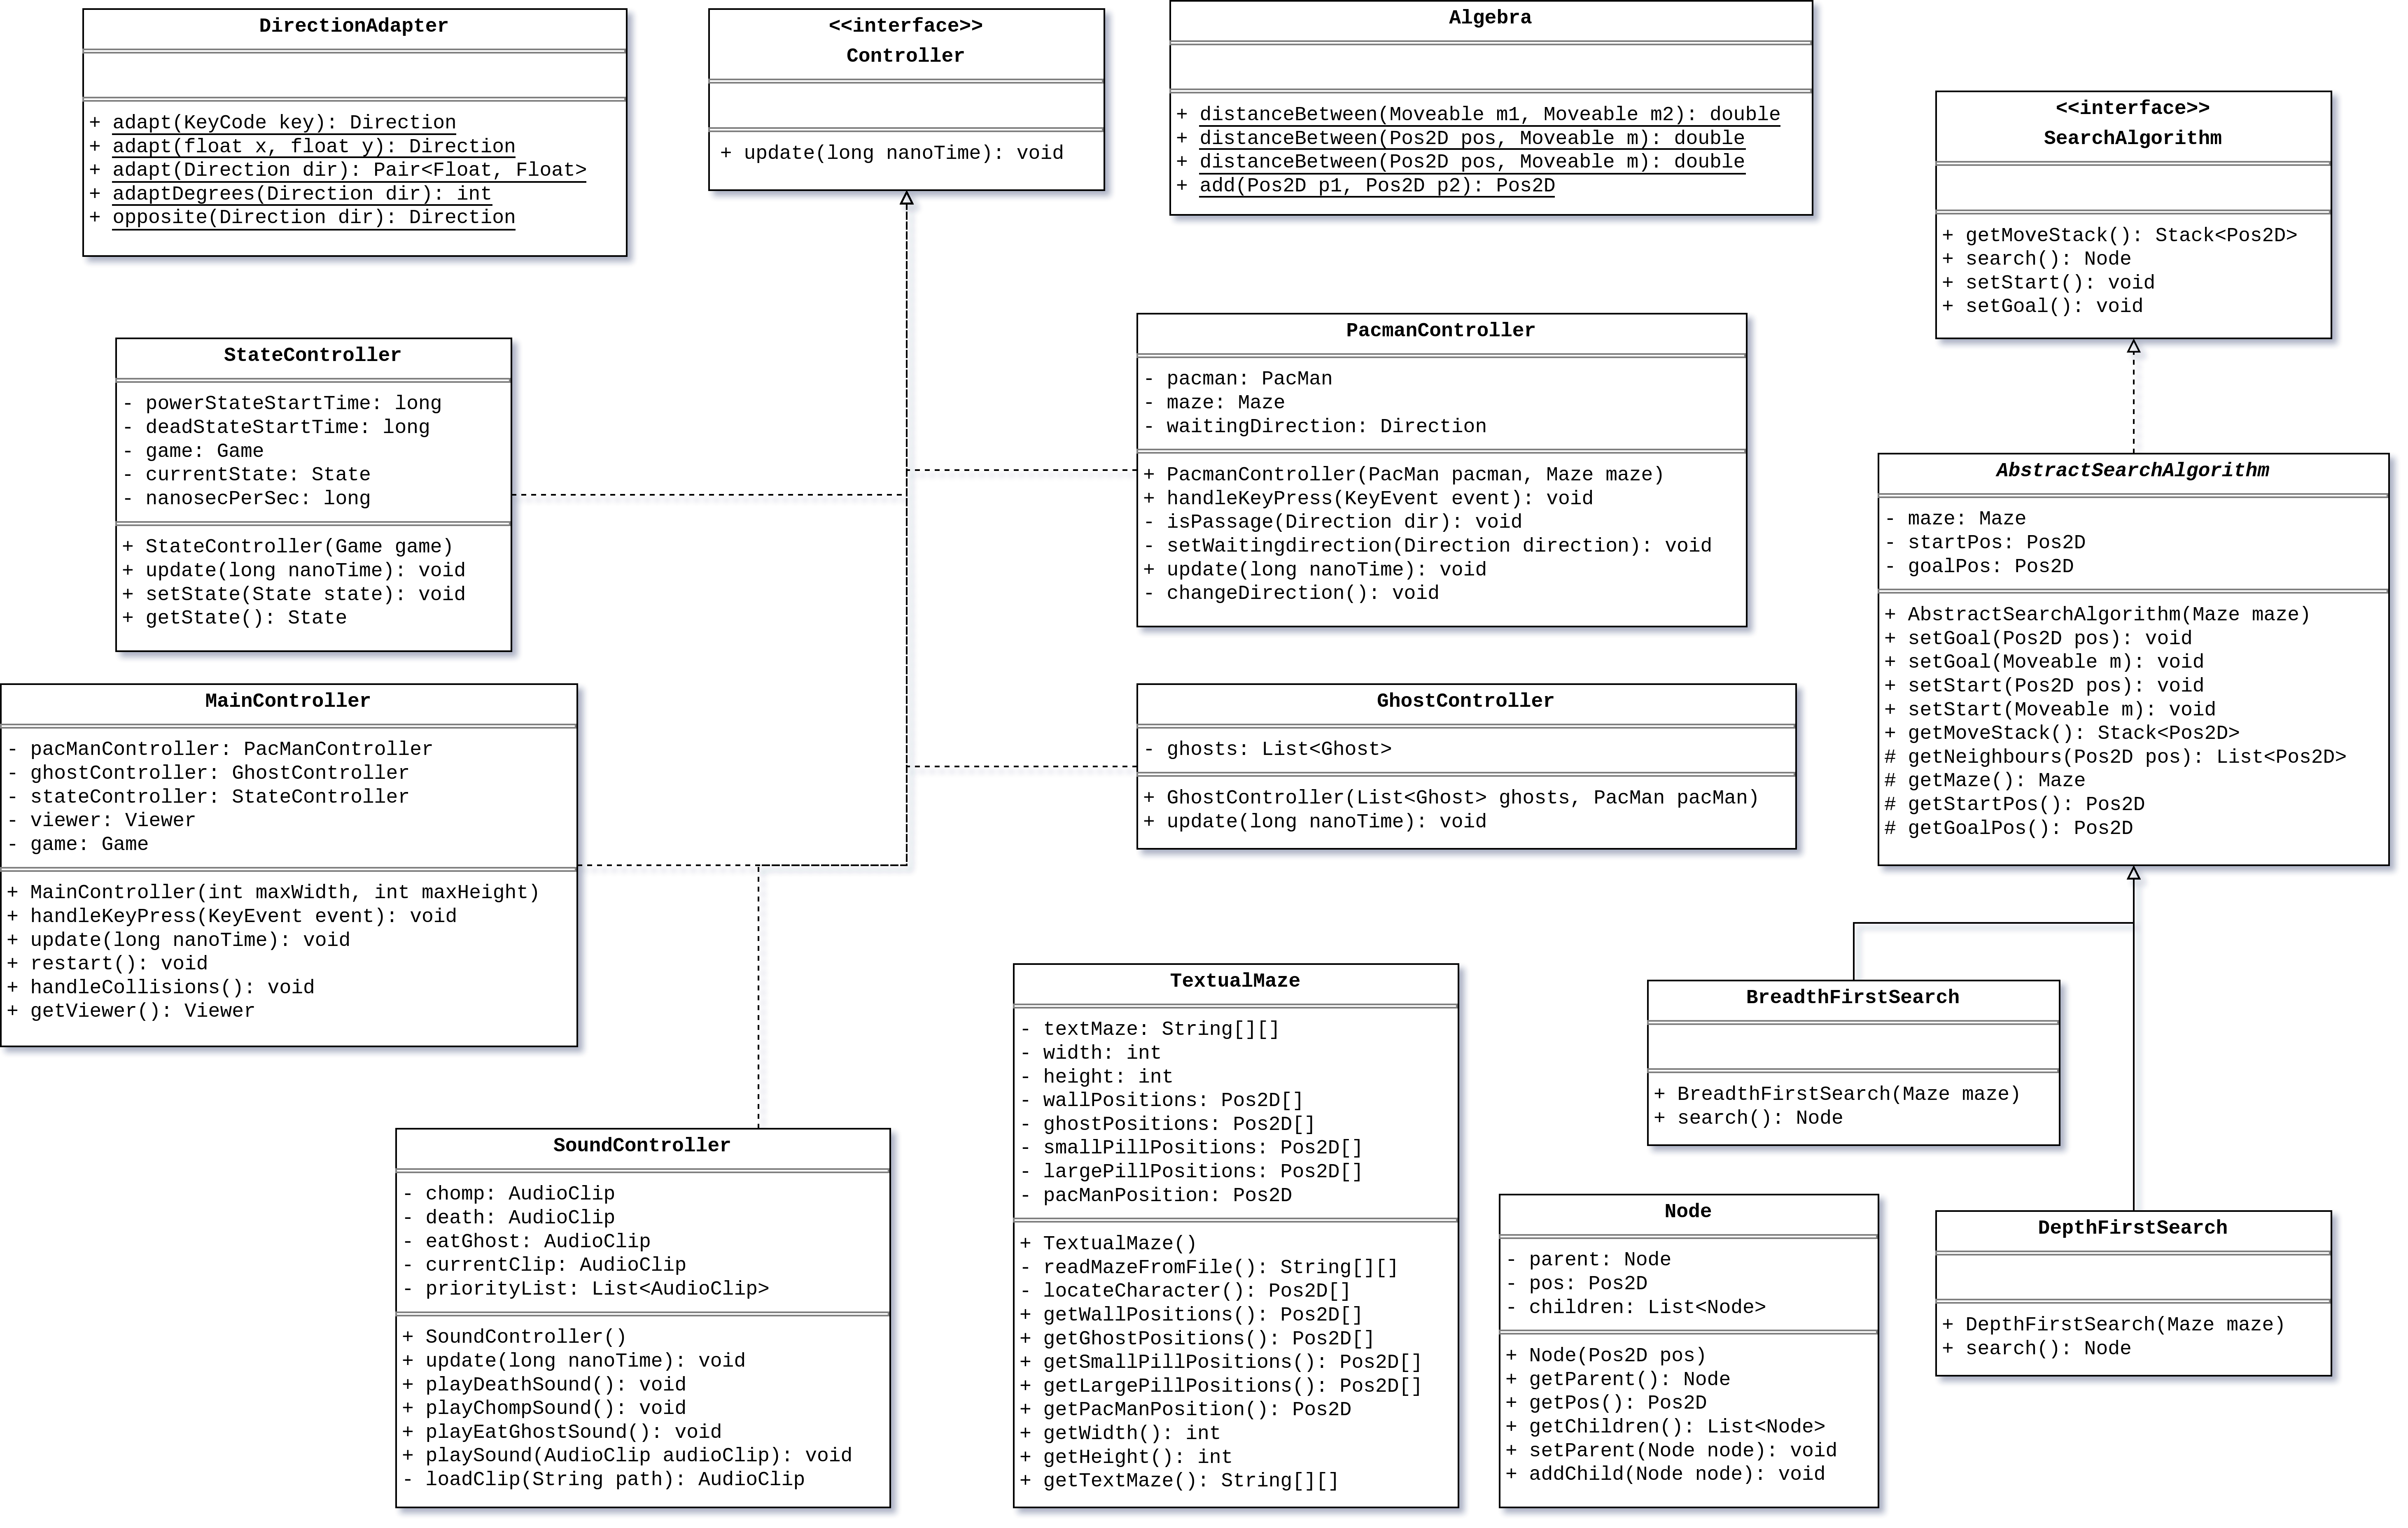
\includegraphics[width=0.95\textwidth]{figures/UML-diagram-controller.png}
    \end{center}
    \caption{UML-diagram til \textit{Controller} delen af projektet.}
    \label{UML-diagram-controller}
\end{figure}

Til \textit{Controller} (se \autoref{UML-diagram-controller}) har vi også lavet
en grænseflade, for at specificerer hvad en "Controller" gør. Derefter har vi
lavet controllers til at styre henholdsvis PacMan, spøgelser og de forskellige
stadier af spillet. Med dette har vi lavet en \code{MainController} som
bestemmer hvornår alle de andre controllers skal opdateres, og hvornår vores
\textit{View} bliver opdateret.
% subsection Controller (end)

\subsection{Ændringer}\label{sub:Ændringer} % (fold)
I løbet af projektet har vores design ændret sig en del. I starten var vores
UML-diagram meget mere simpelt, som kan ses på \autoref{UML-diagram-old}.
Enkeltheden er både grundet de manglende felter og metoder, men også at
kompleksiteten af programmet ikke var blevet realiseret endnu. \code{View} var
bare én enkelt klasse som stod for at tegne alt, og \code{Controller} stod kun
for at tage imod input fra brugeren, og bevæge PacMan i labyrinten. Alt
andet logik til spillet var i \code{Maze}, som gjorde projektet uoverskueligt,
samtidig med at det bryder \textit{SRP}. Da vi så begynde at implementerer mere,
lagde vi mærke til hvor god en idé det ville være at splitte det endnu mere op,
og specialisere klasserne vi laver, som er idéen med \textit{SRP}.
\begin{figure}[H]
    \begin{center}
        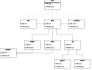
\includegraphics[width=0.95\textwidth]{figures/UML-diagram-old.png}
    \end{center}
    \caption{Det første UML-diagram til projektet.}
    \label{UML-diagram-old}
\end{figure}
I et forsøg på at simplificerer \code{Maze} delte vi den op, og lavede en
\code{Game} klasse, hvis formål var at repræsenterer spillet. På denne måde
kunne \code{Controller} stå for at håndterer alt logikken, som også er mere
typisk af en \textit{Controller} at gøre i \textit{MVC}-modellen. Med denne
ændring ville maze bare stå for at repræsenterer labyrinten. UML-diagrammet for
denne forbedring kan ses på \autoref{UML-diagram-old2}.

\begin{figure}[H]
    \begin{center}
        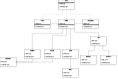
\includegraphics[width=0.95\textwidth]{figures/UML-diagram-old2.png}
    \end{center}
    \caption{Det andet UML-diagram til projektet.}
    \label{UML-diagram-old2}
\end{figure}
Siden da har vi udvidet endnu mere på projektet, og det ser nu ud som det gør på
\autoref{UML-diagram}.
% subsection Ændringer (end)

%\begin{itemize}
%  \item Inkludér et UML-diagram og en beskrivelse af jeres design.
  %\item Giv en kort beskrivelse af jeres diagram:
  %\begin{itemize}
  %  \item Hvad er de forskellige dele?
  %  \item Har I anvendt designmønstre i jeres design? I så fald, hvor i
  %  diagrammet findes disse? Det er ikke et krav at anvende designmøUML-diagram til \textit{Controller} delen af projektet.nstre, men
  %  kan være en god idé.
  %\end{itemize}
  %\item Dokumentér designbeslutninger hvor I har anvendt SOLID, DRY, eller andre
  %OO-principper. 
%  \item Hvis I i løbet af projektet har forfinet jeres design,
%  giv da en kort beskrivelse af hvilke ændringer I har foretaget og hvorfor.
%\end{itemize}
% section design (end)

\section{Implementation}\label{sec:Implementation} % (fold)

States

% \subsection{Moveable}\label{sub:Moveable} % (fold)
% Som nævnt i design sektionen har vi lavet en \code{Moveable} klasse. Det smarte
% ved den er at vi bare kan kalde metoden \code{move()} på en movable, og så
% bevæger den sig i den retning den har fået tildelt. 
% subsection Moveable (end)

\subsection{PacManController}\label{sub:PacManController} % (fold)
Siden vi har gjort at en \textit{Moveable}'s position er beskrevet med decimal
tal, så skal der noget smart logik til for at PacMan kan bevæge sig "smooth"
omkring hjørner i labyrinten, da den består af en masse væge på
heltals-positioner, og PacMan er samme størrelse som væggene, så han passer kun
lige akurat imellem dem.

Idéen er at man kigger frem foran PacMan for at se om der er en passage til den
side man gerne vil hen, indikeret med et tastetryk. Hvis der er en passage
venter controlleren med at dreje PacMan indtil han er lige ved siden af
passagen. Dette har vi gjort ved at gemme retningn i et felt kaldet for
\code{waitingDirection}, og så hver gang \code{PacManController}'s
\code{update()} metode bliver kaldt, så tjekker den om PacMan's position er en
heltalsværdi. Det må nemlig betyde at han nu står foran den passage som der
tidligere blev set. I så fald drejer PacMan nu til retningen af
\code{waitingDirection}. 

Der er også casen hvor PacMan skifter retning til det modsatte af hvad han
bevæger sig. Så kan vi ikke kigge efter en passage der, for det vil der altid
være, og han vil dermed ikke skifte retning med det samme. Så i dette tilfælde
skifter vi bare retning med det samme. Hvis det er sådan at PacMan står stille,
så er vi ikke interreseret i at kigge efter en passage, og han skal bare bevæge
sig i den retning som man trykker med det samme.

For at lave alt dette med retninger, lavede vi en \code{enum} klasse til at
holde styr på de fire retninger vi tillader: op, ned, højre og venstre. For at
finde ud af hvilken en af disse retninger vores tastetryk svarer til, lavede vi
også en \code{DirectionAdapter} klasse, som står for at konverterer imellem
\code{Direction} og andre representationer af en retning.
% subsection PacManController (end)

\subsection{Ghost AI}\label{sub:Ghost AI} % (fold)

% subsection Ghost AI (end)

\subsection{Animationer}\label{sub:Animationer} % (fold)

% subsection Animationer (end)

\begin{itemize}
  \item Formålet med denne rapportsektion er at give den interesserede læser et
  overblik over de interessante implementationsdetaljer, som er værd at kigge
  nærmere på i jeres kodebase, samt nødvendige detaljer for at køre jeres kode.
  \item angiv hvilken version af java i har brugt til at teste og kompilere
  jeres kode, og inkludérkorte instruktioner til hvordan man kompilerer og kører
  koden.
  \item giv en beskrivelse på højniveau af interessante implementationsaspekter.
  F.eks., aspekter, I har brugt særligt meget tid eller energi på.
  \item Det kunne f.eks. være mere avancerede aspekter såsom hvordan I håndterer
  AI, hvordan I håndterer spilhandlinger, animation, eller andet.
  \item Hold beskrivelsen overordnet. Vi kan læse jeres kode for detaljerne.
\end{itemize}
% section Implementation (end)

\newpage
\section{Kvalitetssikring}\label{sec:Kvalitetssikring} % (fold)
Til fordel for at sikre, at vores kode/program/spil lever op til kravsspecifikationen (se \autoref{sec:design}), har vi valgt at anvende unit-tests. Unit-testing defineres i denne kontekst som test af enkelte komponenter af programmet, som til sammen skaber det ønskede overblik.

I overenstemmelse med vores valg af unit-tests, er det også underforstået, at vi tester i en form for white-box testing. Med dette betyder det, at dem der skriver testsne (os som udviklere af spillet i dette tilfælde), kender til alt logikken bag implementeringen. Med dette, har man som "\textit{tester}", altså mulighed for at tjekke, om en given invariant for en given metode overholdes under kørsel.

Mere specifikt; har vi valg at benytte os af \textit{Java}s framework \code{JUnit}, som b.la. understøtter behjælpelige sammenligningsmetoder (f.eks. \textit{assertions} via \code{assert}).

Med dette, anvender vi altså også unit-testing som middel til at krydstjekke med vores kravsspecifikation, om disse (krav) samt eventuelle invarianter er overholdt.

Med anvendelse af ovennævnte, kan fejfindingprocessen under udviklingen, i nogle tilfælde, forkortes markant. Man kan med andre ord, nogle gange, såfremt man skriver tilstrækkelige unit-tests, forsimple samt forbedre design og udviklingsprocessen.

Ydermere, har vi til håndtering af versionsstyring anvendt \code{git} i form af nye branches under udvikling af nye programfunktionaliteter. Dette konstruerer en form for automatiseret testing, da man ikke kan publicere ny funktionalitet, før det passer med den resterende kodebase (f.eks. håndtering af mergeconflicts mm.). Denne form for \textit{automatiseret} testing er også kendt som \textit{Continuous integration testing}.

\textcolor{ocre}{\boxed{\text{INDKLUDER ANDEN TILGANG TIL TEST?}}}

% \begin{itemize}
%   \item Beskriv hvordan I har testet, at jeres kode lever op til
%   kravsspecifikationen. Har I, f.eks., benyttet unit tests? Manuelle tests?
%   \item Ville I have taget en anden tilgang til kvalitetssikring hvis I skulle
%   designe og implementere projektet forfra?
% \end{itemize}
% section Kvalitetssikring (end)

\section{Proces}\label{sec:Proces} % (fold)
\begin{itemize}
  \item Arbejdede I i faser i løbet af projektet?
  \item Hvordan gik samarbejdet, og hvordan sikrede I lige deltagelse?
  \item Brugte I tekniske værktøjer til at få samarbejdet til at glide nemmere
  på tværs af maskiner?
  \item Har I brugt AI som støtte under udviklingen af jeres projekt? I så fald,
  hvordan?
\end{itemize}
% section Proces (end)

\section{Diskussion}\label{sec:Diskussion} % (fold)
\begin{itemize}
  \item Ville I gøre noget anderledes hvis I skulle implementere projektet
  forfra?
  \item Var der dele af projektbeskrivelsen I ikke nåede? I så fald, hvordan er
  disse dele kompatible med jeres design? Ville I foretage ændringer for at
  imødekomme ændringer?
\end{itemize}
% section Diskussion (en

\end{document}
